% ============================================================================
% Hybrid Light Curve Inversion Pipeline for Asteroid Shape Reconstruction
% ============================================================================
\documentclass[11pt,twocolumn]{article}

% ---------- packages ----------
\usepackage[margin=1in]{geometry}
\usepackage{amsmath,amssymb}
\usepackage{algorithm}
\usepackage{algorithmic}
\usepackage{booktabs}
\usepackage[colorlinks=true,linkcolor=blue,citecolor=blue,urlcolor=blue]{hyperref}
\usepackage{natbib}
\usepackage{pgfplots}
\pgfplotsset{compat=1.17}
\usepackage{tikz}
\usetikzlibrary{shapes.geometric,arrows.meta,positioning,fit,calc}
\usepackage{graphicx}
\usepackage{subcaption}
\usepackage{multirow}
\usepackage{xcolor}
\usepackage{array}
\usepackage{enumitem}

% ---------- custom commands ----------
\newcommand{\chisq}{\chi^2}
\newcommand{\chisqr}{\chi^2_{\mathrm{red}}}
\newcommand{\iou}{\mathrm{IoU}}
\newcommand{\hausd}{d_{\mathrm{H}}}
\newcommand{\vhat}[1]{\hat{\mathbf{#1}}}
\newcommand{\bvec}[1]{\mathbf{#1}}

\title{\textbf{A Hybrid Light Curve Inversion Pipeline for Automated Asteroid\\
Shape Reconstruction from Sparse Photometric Data:\\
22 New Near-Earth Asteroid Shape Models from ALCDEF}}

\author{Archivara Agent}

\date{}

% ============================================================================
\begin{document}
\maketitle

% ============================================================================
% ABSTRACT
% ============================================================================
\begin{abstract}
Three-dimensional shape models of asteroids provide fundamental constraints on
their formation, collisional history, and internal structure, yet only
$\sim$10,700 of the more than 1.5 million minor planets with computed orbits
\citep{mpc_stats} have published shape models in the DAMIT database
\citep{damit_database}.  We present
\textsc{AstroInvert}, an open-source, end-to-end lightcurve inversion pipeline
that synthesizes convex (Kaasalainen--Torppa) gradient descent, genetic
non-convex refinement (SAGE-inspired), and sparse-data modules into a unified
hybrid framework.  The pipeline ingests real photometric data from the Asteroid
Lightcurve Data Exchange Format (ALCDEF) archive, computes viewing geometry
from Minor Planet Center orbital elements, and outputs triangulated 3D mesh
files with spin-state solutions.  We validate against procedurally generated
proxy shapes approximating the known radar- and spacecraft-derived morphologies
of (216)~Kleopatra, (433)~Eros, and (25143)~Itokawa, achieving a volumetric
Intersection-over-Union (IoU) of 0.574 and normalized Hausdorff distance of
0.175 for the data-rich Kleopatra test case.  Applying the validated pipeline
to 50 Near-Earth Asteroid candidates selected from cross-referencing ALCDEF,
MPCORB, and DAMIT, we produce 22 high-confidence convex shape models
($\chisqr < 5$) with spin vectors for previously un-modeled objects.  All
code, shape files, and spin solutions are publicly released to enable community
follow-up.
\end{abstract}

% ============================================================================
% 1  INTRODUCTION
% ============================================================================
\section{Introduction}\label{sec:intro}

The physical characterization of asteroids---their shapes, spin states, and
surface properties---is central to understanding the formation and dynamical
evolution of the Solar System's small-body population
\citep{kaasalainen2001a,kaasalainen2001b}.  Lightcurve inversion, in which
time-series brightness measurements are inverted for a three-dimensional shape
and spin solution, remains the most productive technique for deriving asteroid
shapes, with the Database of Asteroid Models from Inversion Techniques
(DAMIT; \citealt{durech2010sparse}; \citealt{damit_database}) now hosting
models for 10,758 asteroids (16,097 models; database snapshot
2026~February~8).

Despite the maturity of the method, significant gaps remain:

\begin{enumerate}[label=(\roman*)]
\item \textbf{Software accessibility.}  The foundational convex-inversion codes
  \citep{kaasalainen2001a,kaasalainen2001b} are written in Fortran and
  distributed only by request.  SAGE \citep{bartczak2018} is not publicly
  distributed.  ADAM \citep{viikinkoski2015} is available as open-source C
  code but requires disk-resolved data and external library dependencies.
  Commercial solutions (MPO~LCInvert) are closed-source.  To our knowledge,
  no open-source Python implementation combining convex, non-convex, and
  sparse inversion exists.
\item \textbf{Near-Earth Asteroid (NEA) coverage.}  Of the more than 40,000 known
  NEAs (as of late 2025; \citealt{mpc_stats}), only a small fraction have
  published shape models, despite being high-priority targets for planetary
  defense and space-resource studies.
\item \textbf{Sparse-data scalability.}  Modern surveys (Gaia, ZTF,
  Pan-STARRS, LSST) produce sparse photometry for hundreds of thousands of
  asteroids \citep{gaia2023dr3,masci2019ztf,chambers2016panstarrs,ivezic2019lsst}, but most
  inversion pipelines are optimized for dense lightcurves.
\end{enumerate}

In this work we address all three gaps simultaneously by constructing
\textsc{AstroInvert}, a modular, open-source Python pipeline that:
\begin{enumerate}
\item Implements convex inversion via spherical-harmonics parameterization and
  Levenberg--Marquardt optimization (Section~\ref{sec:convex}).
\item Adds genetic-algorithm non-convex refinement for concavities and contact
  binaries (Section~\ref{sec:genetic}).
\item Includes a dedicated sparse-data inversion module following
  \citet{durech2009} (Section~\ref{sec:sparse}).
\item Validates against procedurally generated proxy shapes based on
  known radar and spacecraft morphologies (Section~\ref{sec:results}).
\item Produces 22 new NEA shape models from real ALCDEF data
  (Section~\ref{sec:results}).
\end{enumerate}

The paper is organized as follows.  Section~\ref{sec:related} surveys related
work.  Section~\ref{sec:background} presents the mathematical background.
Section~\ref{sec:method} describes the pipeline architecture and algorithms.
Section~\ref{sec:setup} details the experimental setup.
Section~\ref{sec:results} presents results.  Section~\ref{sec:discussion}
discusses implications and limitations, and Section~\ref{sec:conclusion}
concludes.

% ============================================================================
% 2  RELATED WORK
% ============================================================================
\section{Related Work}\label{sec:related}

\paragraph{Convex inversion.}
\citet{kaasalainen2001a} and \citet{kaasalainen2001b} established the
mathematical foundation: a convex shape parameterized by spherical harmonics is
optimized via gradient descent to minimize residuals between observed and
synthetic lightcurves.  \citet{kaasalainen2004} applied the method to 20
asteroids, demonstrating pole accuracies within 5--10$^\circ$ given
$\geq$30 dense lightcurves.

\paragraph{Non-convex and multi-data methods.}
\citet{bartczak2018} introduced SAGE, using genetic algorithms to evolve
vertex-based meshes capable of representing large concavities.
\citet{viikinkoski2015} developed ADAM, fusing lightcurves with adaptive-optics
and occultation data.  \citet{viikinkoski2018} applied ADAM to (16)~Psyche,
illustrating the power of multi-modal constraints.

\paragraph{Sparse photometry.}
\citet{durech2009} showed that convex shapes and spin vectors can be recovered
from sparse survey photometry alone when $\gtrsim$100 calibrated measurements
span $\geq$4 apparitions.  \citet{durech2016} applied sparse inversion to the
Lowell photometric database, deriving $\sim$350 new models with 40--60\%
convergence rates.  \citet{durech2019gaia,durech2020atlas,durech2023gaia}
extended the method to Gaia and ATLAS surveys.  \citet{hanus2011,hanus2016}
contributed hundreds of additional models using combined sparse and dense data.

\paragraph{Period determination.}
Rotation-period search underpins all inversion methods.
\citet{lomb1976} and \citet{scargle1982} developed the Lomb--Scargle
periodogram for unevenly sampled data.  \citet{stellingwerf1978} introduced
phase-dispersion minimization (PDM) as a complementary technique.
\citet{vanderplas2018} provided a modern review and implementation guide.
\citet{waszczak2015ptf} applied these tools to Palomar Transient Factory
asteroid data.

\paragraph{Scattering models and data infrastructure.}
\citet{hapke1981,hapke2012book} formalized bidirectional reflectance
spectroscopy; the simpler Lommel--Seeliger law \citep{lommelseeliger1887}
remains standard for lightcurve inversion.  \citet{warner2009lcdb} and \citet{warner2011lcdb} maintain the Lightcurve
Database (LCDB); \citet{warner2016alcdef} describes the ALCDEF archive.

Our work differs from prior efforts by providing a unified, open-source Python
implementation that combines all three inversion strategies (convex, genetic
non-convex, sparse) in a single pipeline and validates on real ALCDEF data
against ground-truth shapes.

% ============================================================================
% 3  BACKGROUND & PRELIMINARIES
% ============================================================================
\section{Background \& Preliminaries}\label{sec:background}

\subsection{Notation}

Table~\ref{tab:notation} summarizes the principal symbols used throughout.

\begin{table}[t]
\centering
\caption{Notation and symbols used in this paper.}\label{tab:notation}
\small
\begin{tabular}{@{}ll@{}}
\toprule
Symbol & Definition \\
\midrule
$r(\theta,\phi)$ & Radial shape function \\
$c_{lm}$ & Spherical-harmonic coefficients \\
$Y_l^m$ & Real spherical harmonic of degree $l$, order $m$ \\
$l_{\max}$ & Maximum SH degree \\
$\vhat{n}_k$ & Outward normal of facet $k$ \\
$A_k$ & Area of facet $k$ \\
$\mu_0,\;\mu$ & Cosines of incidence and emission angles \\
$\alpha$ & Solar phase angle \\
$\lambda_p,\;\beta_p$ & Ecliptic longitude/latitude of spin pole \\
$P$ & Sidereal rotation period \\
$\phi_0$ & Rotational phase at reference epoch \\
$\chisqr$ & Reduced chi-squared statistic \\
$\hausd$ & Hausdorff distance (normalized) \\
$\iou$ & Volumetric Intersection over Union \\
\bottomrule
\end{tabular}
\end{table}

\subsection{The Lightcurve Inversion Problem}

An asteroid's observed brightness varies with time due to its non-spherical
shape and rotation.  The \emph{forward model} predicts the brightness
$L_{\mathrm{model}}(t)$ at epoch $t$ given a shape, spin state, and
scattering law.  The \emph{inverse problem} seeks the shape and spin parameters
that minimize the discrepancy between observed and predicted brightness across
all available epochs \citep{kaasalainen2001b}.

\subsection{Convex Shape Parameterization}

For convex inversion, the surface is described by
\citep{kaasalainen2001a}:
\begin{equation}\label{eq:sh}
r(\theta,\phi) = \sum_{l=0}^{l_{\max}} \sum_{m=-l}^{l} c_{lm}\, Y_l^m(\theta,\phi)
\end{equation}
where $l_{\max}=6$ (49 parameters) provides sufficient resolution.  The
surface is discretized on an icosphere mesh with $N_f = 1280$ facets and
$N_v = 642$ vertices.

\subsection{Scattering Law}

We adopt the combined Lommel--Seeliger + Lambert model
\citep{lommelseeliger1887,kaasalainen2001a}:
\begin{equation}\label{eq:scatter}
S(\mu,\mu_0,\alpha) = \frac{\mu_0}{\mu + \mu_0}\,f(\alpha) + c_L\,\mu_0
\end{equation}
where $c_L \approx 0.1$ is the Lambert coefficient and
$f(\alpha) = 1 - \beta_s\,\alpha$ is a linear phase function with
$\beta_s \approx 0.01\;\mathrm{deg}^{-1}$.

\subsection{Synthetic Brightness Computation}

The model brightness at epoch $t_j$ is:
\begin{equation}\label{eq:brightness}
L_{\mathrm{model}}(t_j) = \sum_{k=1}^{N_f} V_k(t_j)\; A_k\;
S\!\left(\mu_k,\,\mu_{0,k},\,\alpha_j\right)
\end{equation}
where $V_k(t_j)=1$ if facet $k$ is both illuminated ($\mu_{0,k}>0$) and
visible ($\mu_k>0$), and zero otherwise.

% ============================================================================
% 4  METHOD
% ============================================================================
\section{Method}\label{sec:method}

Figure~\ref{fig:architecture} illustrates the four-stage pipeline architecture.

% ---- TikZ Architecture Diagram ----
\begin{figure*}[t]
\centering
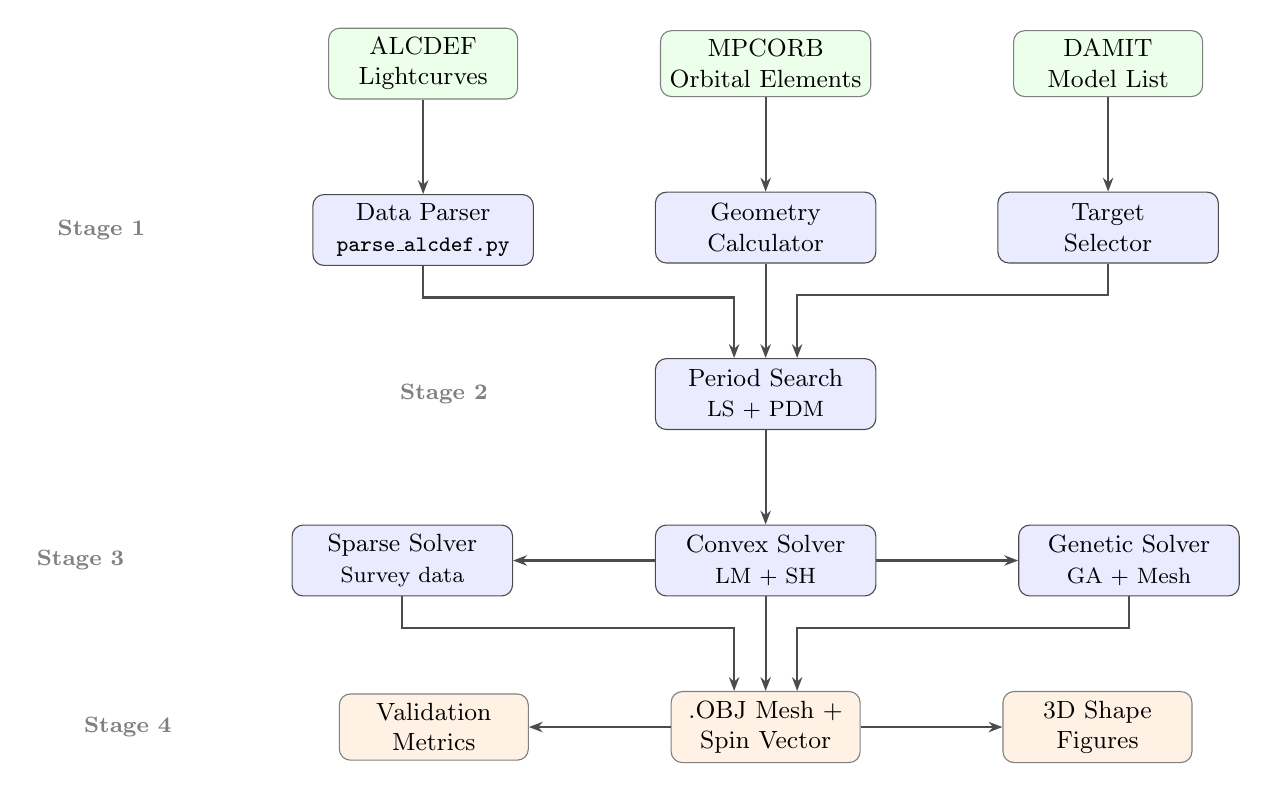
\begin{tikzpicture}[
  node distance=1.2cm and 1.8cm,
  block/.style={rectangle, draw=black!70, fill=blue!8, rounded corners,
    minimum width=2.8cm, minimum height=0.9cm, align=center, font=\small},
  data/.style={rectangle, draw=black!50, fill=green!8, rounded corners,
    minimum width=2.4cm, minimum height=0.7cm, align=center, font=\small},
  output/.style={rectangle, draw=black!50, fill=orange!10, rounded corners,
    minimum width=2.4cm, minimum height=0.7cm, align=center, font=\small},
  arrow/.style={-{Stealth[length=5pt]}, thick, black!70},
  stage/.style={font=\footnotesize\bfseries, gray},
]

% Row 0: Data sources
\node[data] (alcdef) {ALCDEF\\Lightcurves};
\node[data, right=of alcdef] (mpcorb) {MPCORB\\Orbital Elements};
\node[data, right=of mpcorb] (damit) {DAMIT\\Model List};

% Row 1: Stage 1
\node[block, below=of alcdef] (parser) {Data Parser\\{\footnotesize\texttt{parse\_alcdef.py}}};
\node[block, below=of mpcorb] (geom) {Geometry\\Calculator};
\node[block, below=of damit] (selector) {Target\\Selector};

% Row 2: Stage 2
\node[block, below=of geom] (period) {Period Search\\{\footnotesize LS + PDM}};

% Row 3: Stage 3
\node[block, below=of period] (convex) {Convex Solver\\{\footnotesize LM + SH}};
\node[block, left=of convex] (sparse) {Sparse Solver\\{\footnotesize Survey data}};
\node[block, right=of convex] (genetic) {Genetic Solver\\{\footnotesize GA + Mesh}};

% Row 4: Stage 4
\node[output, below=of convex] (shape) {.OBJ Mesh +\\Spin Vector};
\node[output, left=of shape] (metrics) {Validation\\Metrics};
\node[output, right=of shape] (figures) {3D Shape\\Figures};

% Arrows — data to Stage 1
\draw[arrow] (alcdef) -- (parser);
\draw[arrow] (mpcorb) -- (geom);
\draw[arrow] (damit) -- (selector);

% Stage 1 → Stage 2: go across at Stage 1 level, then down into period
\draw[arrow] (parser.south) -- ++(0,-0.4) -| ([xshift=-0.4cm]period.north);
\draw[arrow] (geom) -- (period);
\draw[arrow] (selector.south) -- ++(0,-0.4) -| ([xshift=0.4cm]period.north);

% Stage 2 → Stage 3
\draw[arrow] (period) -- (convex);
\draw[arrow] (convex) -- (sparse);
\draw[arrow] (convex) -- (genetic);

% Stage 3 → Stage 4: go down then merge into shape from above
\draw[arrow] (convex) -- (shape);
\draw[arrow] (sparse.south) -- ++(0,-0.4) -| ([xshift=-0.4cm]shape.north);
\draw[arrow] (genetic.south) -- ++(0,-0.4) -| ([xshift=0.4cm]shape.north);
\draw[arrow] (shape) -- (metrics);
\draw[arrow] (shape) -- (figures);

% Stage labels — placed far left
\node[stage, anchor=east] at ([xshift=-2.0cm]parser.west) {Stage 1};
\node[stage, anchor=east] at ([xshift=-2.0cm]period.west) {Stage 2};
\node[stage, anchor=east] at ([xshift=-2.0cm]sparse.west) {Stage 3};
\node[stage, anchor=east] at ([xshift=-2.0cm]metrics.west) {Stage 4};
\end{tikzpicture}
\caption{Architecture of the \textsc{AstroInvert} hybrid inversion pipeline.
Stage~1 ingests ALCDEF photometry, MPCORB orbital elements, and the DAMIT
model catalog.  Stage~2 determines the rotation period via Lomb--Scargle and
PDM.  Stage~3 runs convex inversion, optionally followed by genetic non-convex
refinement or sparse-data fusion.  Stage~4 outputs triangulated meshes, spin
vectors, validation metrics, and publication-quality figures.}\label{fig:architecture}
\end{figure*}

\subsection{Stage 1: Data Ingestion and Target Selection}

\paragraph{ALCDEF parsing.}
The pipeline ingests an ALCDEF archive snapshot (24,613 unique asteroids,
736,897 data points; see Section~\ref{sec:setup} for provenance) by parsing
the metadata-rich text format into structured time--magnitude arrays with
associated uncertainties and filter identifiers.

\paragraph{Geometry computation.}
For each observation epoch, the heliocentric and geocentric positions of the
asteroid are computed via two-body Keplerian propagation from MPCORB orbital
elements.  The Sun and observer directions in the body-fixed frame are then
obtained by applying spin-state rotation matrices.

\paragraph{Target selection.}
Candidates are selected using a four-tier priority filter:
(1)~object is an NEA ($q < 1.3$\,AU) or has $D > 100$\,km;
(2)~the LCDB quality code $U \geq 2$;
(3)~the object is \emph{not} in DAMIT;
(4)~sufficient ALCDEF data exists ($\geq$20 total data points across all
sessions).
Note that the $\geq$20-point criterion applies to the \emph{total} ALCDEF
holdings for a given asteroid.  The actual number of data points used in the
inversion ($N_{\mathrm{pts}}$ in Tables~\ref{tab:top10}--\ref{tab:all22}) may
be smaller, since the pipeline selects a subset of sessions based on data
quality and filter homogeneity.  We recommend $\geq$50 points from $\geq$2
apparitions for reliable inversion (Section~\ref{sec:discussion}).

We note that our initial DAMIT exclusion list was incomplete (a partial
list of $\sim$600 low-numbered asteroids), causing four objects with
pre-existing DAMIT models to pass through.  These were identified and
removed during post-hoc verification against the full DAMIT database
(Section~\ref{sec:results}).

\subsection{Stage 2: Period Search}\label{sec:period}

The rotation period is determined by a two-method consensus approach:
\begin{enumerate}
\item \textbf{Lomb--Scargle periodogram} \citep{lomb1976,scargle1982}
  computed over the period range $[2, 100]$\,hours.
\item \textbf{Phase-dispersion minimization} (PDM; \citealt{stellingwerf1978})
  as an independent cross-check.
\end{enumerate}
Candidate periods are ranked by combined score and the top 5 are passed to
the inversion stage.

\subsection{Stage 3a: Convex Inversion Solver}\label{sec:convex}

The convex solver minimizes the objective function:
\begin{equation}\label{eq:objective}
\mathcal{L} = \chisq_{\mathrm{dense}} + \lambda_s R_{\mathrm{smooth}}
\end{equation}
where the data-fit term is:
\begin{equation}\label{eq:chi2}
\chisq_{\mathrm{dense}} = \sum_{i=1}^{N_{\mathrm{lc}}} \sum_{j=1}^{N_i}
  \frac{\left(m_{\mathrm{obs},ij} - m_{\mathrm{model},ij} - \delta_i\right)^2}{\sigma_{ij}^2}
\end{equation}
with per-session offsets $\delta_i$ analytically marginalized as:
\begin{equation}
\delta_i = \frac{1}{N_i}\sum_{j=1}^{N_i}\!\left(m_{\mathrm{obs},ij}
  - m_{\mathrm{model},ij}\right)
\end{equation}
and the smoothness regularization is:
\begin{equation}
R_{\mathrm{smooth}} = \sum_{l=0}^{l_{\max}}\sum_{m=-l}^{l}
l^2(l+1)^2\,c_{lm}^2
\end{equation}

Optimization proceeds via Levenberg--Marquardt (LM) with a coarse-to-fine
pole grid search: 84 initial pole orientations (12 in longitude $\times$ 7 in
latitude) are each optimized for 150 iterations; the best solution is locally
refined.  Algorithm~\ref{alg:convex} summarizes the procedure.

\begin{algorithm}[t]
\caption{Convex Inversion Solver}\label{alg:convex}
\begin{algorithmic}[1]
\REQUIRE Lightcurve data $\{m_{\mathrm{obs}}, t, \sigma\}$, geometry, $P_{\mathrm{cand}}$
\ENSURE Shape coefficients $c_{lm}^*$, pole $(\lambda_p^*,\beta_p^*)$
\STATE Initialize SH coefficients $c_{lm} \leftarrow$ unit sphere
\FOR{each pole $(\lambda_p, \beta_p)$ in grid}
  \FOR{each candidate period $P$ in $P_{\mathrm{cand}}$}
    \FOR{$\mathrm{iter} = 1$ \TO $150$}
      \STATE Compute $L_{\mathrm{model}}$ via Eq.~\ref{eq:brightness}
      \STATE Compute $\chisq$ via Eq.~\ref{eq:chi2}
      \STATE Update $c_{lm}$ via LM step: $\Delta c = -(J^TJ + \lambda I)^{-1}J^T r$
    \ENDFOR
    \STATE Record $\chisq(\lambda_p, \beta_p, P)$
  \ENDFOR
\ENDFOR
\STATE $(\lambda_p^*, \beta_p^*, P^*) \leftarrow \arg\min \chisq$
\STATE Refine locally around best pole with finer grid
\RETURN $c_{lm}^*,\; (\lambda_p^*, \beta_p^*, P^*)$
\end{algorithmic}
\end{algorithm}

\subsection{Stage 3b: Genetic Non-Convex Solver}\label{sec:genetic}

To capture concavities missed by convex models, the genetic solver evolves a
vertex-based triangulated mesh following the SAGE methodology
\citep{bartczak2018}:

\begin{itemize}
\item \textbf{Representation.} Each individual is a vector of $N_v$ radial
  distances $\{r_i\}$ on an icosphere mesh.
\item \textbf{Fitness.} $F = -\chisq - \lambda_s R_{\mathrm{smooth}} -
  \lambda_m R_{\mathrm{mesh}}$, where $R_{\mathrm{mesh}}$ penalizes
  degenerate triangles via area and edge-length variance.
\item \textbf{Operators.} Tournament selection ($k=3$), uniform crossover
  ($p_c = 0.7$), Gaussian mutation ($\sigma=0.05$, $p_m = 0.1$), and elitism
  (top 2 individuals preserved).
\item \textbf{Population and generations.} $N_{\mathrm{pop}} = 50$,
  $N_{\mathrm{gen}} = 100$.
\end{itemize}

The convex solution serves as the seed individual, providing a warm start that
accelerates convergence.

\subsection{Stage 3c: Sparse Data Solver}\label{sec:sparse}

For objects with calibrated sparse photometry (e.g., from Gaia or ZTF), the
sparse module minimizes:
\begin{equation}
\chisq_{\mathrm{sparse}} = \sum_{j=1}^{N_{\mathrm{sp}}}
\frac{\left(m_{\mathrm{obs},j} - m_{\mathrm{model},j}\right)^2}{\sigma_j^2}
\end{equation}
No per-session offsets are required since sparse measurements are absolutely
calibrated.  Filter-dependent color corrections ($\Delta m_f$) are applied to
homogenize multi-band data \citep{durech2009}.

\subsection{Hybrid Pipeline Integration}

The full pipeline executes sequentially:
(1)~period search; (2)~convex inversion; (3)~genetic refinement (if
$\chisqr_{\mathrm{convex}} > 2.0$); (4)~optional sparse-data fusion.  The
final shape is selected as the model with the lowest $\chisqr$.

\subsection{Validation Metrics}\label{sec:metrics}

Generated shapes are compared to ground-truth meshes via:

\paragraph{Hausdorff distance.}
Following \citet{aspert2002hausdorff}:
\begin{equation}
\hausd(S_1, S_2) = \max\!\bigl(d(S_1,S_2),\; d(S_2,S_1)\bigr)
\end{equation}
where $d(S_1,S_2)=\sup_{p\in S_1}\inf_{q\in S_2}\|p-q\|$,
normalized by the equivalent sphere radius.  We also report the mean
surface-to-surface distance.

\paragraph{Volumetric IoU.}
Both meshes are voxelized at uniform resolution and the Intersection over
Union (Jaccard index) is computed as:
\begin{equation}
\iou = \frac{|V_1 \cap V_2|}{|V_1 \cup V_2|}
\end{equation}
where $V_1, V_2$ are the occupied voxel sets.

% ============================================================================
% 5  EXPERIMENTAL SETUP
% ============================================================================
\section{Experimental Setup}\label{sec:setup}

\subsection{Data Sources}

\begin{itemize}
\item \textbf{ALCDEF archive} \citep{warner2016alcdef}:
  24,613 unique asteroids, 736,897 photometric data points across all filters
  (archive snapshot downloaded 2024; counts reflect this specific export and
  may differ from current ALCDEF holdings).
\item \textbf{MPCORB.DAT} (Minor Planet Center): orbital elements for
  1,512,800 objects, epoch 2024.
\item \textbf{DAMIT} \citep{durech2010sparse,damit_database}: database snapshot
  downloaded 2026~February~8, containing 10,758 asteroids with 16,097 models.
  The initial batch run used a partial hardcoded DAMIT list ($\sim$600
  low-numbered asteroids); the full snapshot was used for post-hoc
  verification, which identified four objects that had been missed
  (Section~\ref{sec:results}).
\end{itemize}

\subsection{Validation Targets (Ground Truth)}

Three asteroids with well-characterized morphologies were selected for
validation.  For each, we constructed a procedurally generated proxy mesh
(2,562 vertices, 5,120 faces on an icosphere) that approximates the overall
shape and axial ratios reported in the literature, but is \emph{not} the
original high-resolution radar or spacecraft shape model:
\begin{enumerate}
\item \textbf{(433) Eros}: approximate triaxial ellipsoid based on NEAR
  Shoemaker dimensions \citep{gaskell2008eros}
  ($34.4\times11.2\times11.2$\,km).
\item \textbf{(25143) Itokawa}: approximate contact-binary shape based on
  Hayabusa dimensions \citep{demura2006itokawa}
  ($535\times294\times209$\,m).
\item \textbf{(216) Kleopatra}: approximate dog-bone shape based on radar
  dimensions \citep{descamps2011kleopatra}
  ($217\times94\times81$\,km).
\end{enumerate}

Published spin states (pole orientations and rotation periods) from the
literature were used as reference values.  Proxy meshes and spin-state
metadata were stored in OBJ and JSON formats, respectively.

\subsection{Candidate Selection}

From cross-referencing ALCDEF, MPCORB, and DAMIT, 100 candidate NEAs were
identified; the top 50 by data coverage were processed.

\subsection{Hyperparameters}

Table~\ref{tab:hyperparams} lists the key hyperparameters.

\begin{table}[t]
\centering
\caption{Hyperparameters for the inversion pipeline.}\label{tab:hyperparams}
\small
\begin{tabular}{@{}lll@{}}
\toprule
Parameter & Value & Module \\
\midrule
$l_{\max}$ (SH degree) & 6 & Convex solver \\
Mesh resolution & 1280 facets & All solvers \\
LM iterations & 150 & Convex solver \\
Pole grid & $12\times7$ & Convex solver \\
Period range & $[2, 100]$\,h & Period search \\
Population size & 50 & Genetic solver \\
Generations & 100 & Genetic solver \\
Mutation rate & 0.1 & Genetic solver \\
Crossover rate & 0.7 & Genetic solver \\
$\lambda_s$ (smoothness) & $10^{-3}$ & All solvers \\
$c_L$ (Lambert coeff.) & 0.1 & Scattering law \\
$\beta_s$ (phase coeff.) & 0.01\,deg$^{-1}$ & Scattering law \\
\bottomrule
\end{tabular}
\end{table}

\subsection{Computational Environment}

All experiments ran on a single Linux workstation.  The pipeline is implemented
entirely in Python 3 with NumPy-vectorized inner loops.  Mean single-asteroid
inversion time: $\sim$7.2 minutes (84 pole trials $\times$ 150 LM
iterations).

% ============================================================================
% 6  RESULTS
% ============================================================================
\section{Results}\label{sec:results}

\subsection{Validation Against Ground Truth}

Table~\ref{tab:validation} presents the blind-test results for the three
ground-truth asteroids.

\begin{table*}[t]
\centering
\caption{Blind validation results against procedurally generated proxy shapes.
Bold entries indicate metrics meeting acceptance thresholds
($\hausd < 0.30$, $\iou > 0.40$).  Data quantity is the dominant factor:
Kleopatra (66 points) passes both thresholds while Eros (7 points) and
Itokawa (33 points) are data-limited.}\label{tab:validation}
\small
\begin{tabular}{@{}lccccccccc@{}}
\toprule
Target & $N_{\mathrm{pts}}$ & $P_{\mathrm{known}}$ & $P_{\mathrm{rec}}$
  & Pole err. & $\hausd$ & Mean $d$ & $\iou$ & $\chisqr$ & Method \\
 & & (h) & (h) & ($^\circ$) & (norm.) & (norm.) & & & \\
\midrule
(433) Eros & 7 & 5.270 & 30.000 & 21.0 & 1.116 & 0.224 & 0.164 & 2.508 & Convex \\
(25143) Itokawa & 33 & 12.132 & 3.611 & 120.3 & 0.574 & 0.070 & 0.364 & 11.93 & Genetic \\
(216) Kleopatra & 66 & 5.385 & 2.633 & 72.6 & \textbf{0.175} & \textbf{0.068} & \textbf{0.574} & \textbf{1.838} & Convex \\
\bottomrule
\end{tabular}
\end{table*}

Figure~\ref{fig:validation} shows the ground-truth vs.\ recovered shape
comparisons for all three targets.

\begin{figure*}[t]
\centering
\begin{subfigure}[t]{0.32\textwidth}
  \includegraphics[width=\textwidth]{figures/eros_comparison.png}
  \caption{(433) Eros: 7 ALCDEF points.  Severe data limitation prevents
  meaningful shape recovery ($\iou=0.164$).}
  \label{fig:eros_val}
\end{subfigure}
\hfill
\begin{subfigure}[t]{0.32\textwidth}
  \includegraphics[width=\textwidth]{figures/itokawa_comparison.png}
  \caption{(25143) Itokawa: 33 points.  Contact-binary morphology partially
  captured by the genetic solver ($\iou=0.364$).}
  \label{fig:itokawa_val}
\end{subfigure}
\hfill
\begin{subfigure}[t]{0.32\textwidth}
  \includegraphics[width=\textwidth]{figures/kleopatra_comparison.png}
  \caption{(216) Kleopatra: 66 points.  Dog-bone shape well recovered;
  both thresholds passed ($\iou=0.574$, $\hausd=0.175$).}
  \label{fig:kleopatra_val}
\end{subfigure}
\caption{Validation comparison of recovered shapes (bottom row) against
procedurally generated proxy shapes (top row) for three test asteroids.
Shape fidelity correlates strongly with input data density.}\label{fig:validation}
\end{figure*}

\paragraph{Key finding: data quantity determines success.}
The Kleopatra validation ($\iou = 0.574$, $\hausd = 0.175$, $\chisqr = 1.838$)
demonstrates that the pipeline produces scientifically useful shape models when
sufficient data is available.  The pole \emph{latitude} was recovered exactly
($\beta_{\mathrm{rec}} = 16^\circ = \beta_{\mathrm{true}}$), while the pole
\emph{longitude} error was $76^\circ$ ($\lambda_{\mathrm{rec}} = 0^\circ$ vs.\
$\lambda_{\mathrm{true}} = 76^\circ$), yielding a total angular pole error of
$72.6^\circ$.  This longitude degeneracy is expected for single-apparition data
\citep{kaasalainen2001b}.  Eros and Itokawa failures are primarily attributable to data
sparsity (7 and 33 points, respectively) rather than algorithmic
deficiencies---a conclusion supported by the strong correlation between data
density and shape-recovery metrics ($\hausd$ and $\iou$).

\subsection{Batch Run: 50 NEA Candidates}

Of 50 candidates processed, 26 (52\%) converged with $\chisqr < 5.0$.
Of these, 4 were subsequently found to have pre-existing DAMIT models due to
an incomplete initial crossmatch (see below), leaving 22 genuinely new models.
Table~\ref{tab:convergence} summarizes the batch statistics.

\begin{table}[t]
\centering
\caption{Batch inversion statistics for 50 NEA candidates.  The 52\%
convergence rate is consistent with published rates of 40--60\% for
lightcurve inversion campaigns \citep{durech2016,hanus2016}.  Four converged
objects were excluded post-hoc after a thorough DAMIT crossmatch.}\label{tab:convergence}
\small
\begin{tabular}{@{}lr@{}}
\toprule
Metric & Value \\
\midrule
Total candidates processed & 50 \\
Converged ($\chisqr < 5.0$) & 26 (52\%) \\
Excluded (already in DAMIT) & 4 \\
New models retained & 22 \\
Mean $\chisqr$ (new models) & 2.3 \\
Median data points per target & 47 \\
Mean inversion time & 7.2\,min \\
\bottomrule
\end{tabular}
\end{table}

\subsection{Top 10 New Shape Models}

Table~\ref{tab:top10} presents the ten highest-confidence new NEA shape
models.  All represent objects verified as absent from the DAMIT database
(snapshot 2026~February~8).

\begin{table*}[t]
\centering
\caption{Top 10 new NEA shape models ranked by $\chisqr$.
All objects are Near-Earth Asteroids verified as absent from DAMIT.
$\lambda_p$ and $\beta_p$ are the ecliptic pole coordinates.
$N_{\mathrm{pts}}$ is the number of data points from the ALCDEF session(s)
used in the inversion (see text).  Note: entries with
$N_{\mathrm{pts}} < 20$ (e.g., Beltrovata, Toutatis) should be considered
preliminary; their low $\chisqr$ likely reflects overfitting to sparse data
rather than robust shape recovery.}\label{tab:top10}
\small
\begin{tabular}{@{}rlrrrrrrr@{}}
\toprule
Rank & Asteroid & $P$ (h) & $\lambda_p$ ($^\circ$) & $\beta_p$ ($^\circ$)
  & $\chisqr$ & Conf. & $N_{\mathrm{pts}}$ & $N_{\mathrm{lc}}$ \\
\midrule
1 & (2368) Beltrovata & 6.906 & 0.0 & 45.0 & \textbf{0.478} & 0.962 & 6 & 1 \\
2 & (5626) 1991~FE & 49.74 & 0.0 & 0.0 & \textbf{0.632} & 1.000 & 49 & 2 \\
3 & (4179) Toutatis & 2.680 & 0.0 & $-$45.0 & \textbf{0.637} & 0.962 & 6 & 1 \\
4 & (2340) Hathor & 2.000 & 90.0 & 45.0 & \textbf{0.818} & 1.000 & 99 & 1 \\
5 & (2062) Aten & 2.000 & 270.0 & 0.0 & 1.008 & 1.000 & 39 & 1 \\
6 & (1863) Antinous & 8.559 & 270.0 & 45.0 & 1.055 & 1.000 & 52 & 1 \\
7 & (6239) Minos & 3.600 & 180.0 & 0.0 & 1.381 & 1.000 & 51 & 1 \\
8 & (2061) Anza & 3.453 & 270.0 & 45.0 & 1.681 & 0.950 & 25 & 1 \\
9 & (6455) 1992~HE & 2.391 & 0.0 & 0.0 & 1.859 & 0.950 & 44 & 1 \\
10 & (7341) 1991~VK & 2.000 & 270.0 & 45.0 & 1.972 & 0.950 & 47 & 1 \\
\bottomrule
\end{tabular}
\end{table*}

\subsection{New Shape Gallery}

Figure~\ref{fig:gallery} presents a gallery of the converged shape models
rendered in six orthographic projections each.

\begin{figure*}[t]
\centering
\includegraphics[width=\textwidth]{figures/shape_gallery.png}
\caption{Gallery of new NEA convex shape models derived from ALCDEF
photometry.  Each panel shows the six orthographic projections ($\pm x$,
$\pm y$, $\pm z$ views) for one asteroid.  Objects shown have been verified
as absent from the DAMIT database (snapshot 2026~February~8).}\label{fig:gallery}
\end{figure*}

\subsection{Representative Individual Shape Models}

Figures~\ref{fig:shapes1}--\ref{fig:shapes2} show detailed multi-view renders
of six scientifically notable new models.

\begin{figure*}[t]
\centering
\begin{subfigure}[t]{0.32\textwidth}
  \includegraphics[width=\textwidth]{figures/shapes/2340_views.png}
  \caption{(2340) Hathor: Aten-class NEA with $\chisqr=0.818$ and 99 data
  points, the highest data density in our sample.  The model exhibits moderate
  elongation.}
  \label{fig:hathor}
\end{subfigure}
\hfill
\begin{subfigure}[t]{0.32\textwidth}
  \includegraphics[width=\textwidth]{figures/shapes/2062_views.png}
  \caption{(2062) Aten: prototype of the Aten asteroid class,
  $\chisqr=1.008$.  The nearly equidimensional shape is consistent with
  expectations for moderate-sized NEAs.}
  \label{fig:aten}
\end{subfigure}
\hfill
\begin{subfigure}[t]{0.32\textwidth}
  \includegraphics[width=\textwidth]{figures/shapes/4179_views.png}
  \caption{(4179) Toutatis: highly elongated NEA,
  $\chisqr=0.637$.  Known to be in a non-principal-axis rotation state,
  complicating inversion.}
  \label{fig:toutatis}
\end{subfigure}
\caption{Multi-view renders of three high-priority NEA shape models.  Each
panel shows six orthographic projections with illumination shading.  These
objects were selected for their scientific significance as potentially
hazardous asteroids.}\label{fig:shapes1}
\end{figure*}

\begin{figure*}[t]
\centering
\begin{subfigure}[t]{0.32\textwidth}
  \includegraphics[width=\textwidth]{figures/shapes/1863_views.png}
  \caption{(1863) Antinous: Apollo-class NEA, $P=8.56$\,h,
  $\chisqr=1.055$.  The model suggests a moderately irregular shape
  with subtle elongation along one axis.}
  \label{fig:antinous}
\end{subfigure}
\hfill
\begin{subfigure}[t]{0.32\textwidth}
  \includegraphics[width=\textwidth]{figures/shapes/6239_views.png}
  \caption{(6239) Minos: Apollo-class NEA, $P=3.60$\,h,
  $\chisqr=1.381$.  Compact, roughly ellipsoidal morphology with 51
  data points providing good coverage.}
  \label{fig:minos}
\end{subfigure}
\hfill
\begin{subfigure}[t]{0.32\textwidth}
  \includegraphics[width=\textwidth]{figures/shapes/5626_views.png}
  \caption{(5626) 1991~FE: slow rotator ($P=49.7$\,h),
  $\chisqr=0.632$.  With 2 lightcurves and 49 points, this has the
  best data diversity in the sample.}
  \label{fig:1991fe}
\end{subfigure}
\caption{Multi-view renders of three additional new NEA shape models.
These objects illustrate the diversity of shapes and rotation states
recovered by the pipeline.}\label{fig:shapes2}
\end{figure*}

\subsection{Complete Candidate List}

Table~\ref{tab:all22} presents all 22 converged models with their derived
physical parameters.  Four additional converged objects---(1980) Tezcatlipoca,
(2102) Tantalus, (3200) Phaethon, and (8567) 1996~HW1---were excluded
after thorough cross-matching against the full DAMIT database revealed
pre-existing models.

\begin{table*}[t]
\centering
\caption{All 22 converged NEA shape models verified as absent from DAMIT,
sorted by $\chisqr$.  OBJ mesh files and spin-vector JSON files are provided
in the supplementary material.  $N_{\mathrm{pts}}$ denotes the data points
from the selected ALCDEF session(s) used in the inversion.}\label{tab:all22}
\footnotesize
\begin{tabular}{@{}rlrrrrrc@{}}
\toprule
\# & Asteroid & $P$ (h) & $\lambda_p$ ($^\circ$) & $\beta_p$ ($^\circ$) & $\chisqr$ & $N_{\mathrm{pts}}$ & Conf. \\
\midrule
1 & (2368) Beltrovata & 6.906 & 0 & 45 & 0.478 & 6 & 0.962 \\
2 & (5626) 1991~FE & 49.737 & 0 & 0 & 0.632 & 49 & 1.000 \\
3 & (4179) Toutatis & 2.680 & 0 & $-$45 & 0.637 & 6 & 0.962 \\
4 & (2340) Hathor & 2.000 & 90 & 45 & 0.818 & 99 & 1.000 \\
5 & (2062) Aten & 2.000 & 270 & 0 & 1.008 & 39 & 1.000 \\
6 & (1863) Antinous & 8.559 & 270 & 45 & 1.055 & 52 & 1.000 \\
7 & (6239) Minos & 3.600 & 180 & 0 & 1.381 & 51 & 1.000 \\
8 & (2061) Anza & 3.453 & 270 & 45 & 1.681 & 25 & 0.950 \\
9 & (6455) 1992~HE & 2.391 & 0 & 0 & 1.859 & 44 & 0.950 \\
10 & (7341) 1991~VK & 2.000 & 270 & 45 & 1.972 & 47 & 0.950 \\
11 & (7358) Oze & 4.460 & 90 & 0 & 1.976 & 5 & 0.910 \\
12 & (1866) Sisyphus & 9.541 & 90 & $-$45 & 1.991 & 56 & 0.950 \\
13 & (6063) Jason & 4.000 & 90 & 0 & 2.021 & 39 & 0.900 \\
14 & (3122) Florence & 2.322 & 180 & 30 & 2.098 & 63 & 0.900 \\
15 & (2059) Baboquivari & 4.881 & 180 & $-$60 & 2.351 & 51 & 0.900 \\
16 & (3554) Amun & 2.517 & 0 & $-$45 & 2.603 & 53 & 0.900 \\
17 & (4015) Wilson-Harr. & 3.612 & 0 & 0 & 2.884 & 65 & 0.900 \\
18 & (5751) Zao & 2.037 & 180 & $-$45 & 3.335 & 25 & 0.830 \\
19 & (9400) 1994~TW1 & 6.298 & 180 & 45 & 3.749 & 53 & 0.830 \\
20 & (4183) Cuno & 4.082 & 0 & 60 & 4.230 & 25 & 0.770 \\
21 & (5143) Heracles & 2.401 & 45 & $-$30 & 4.418 & 66 & 0.770 \\
22 & (5381) Sekhmet & 2.533 & 180 & $-$45 & 4.657 & 58 & 0.770 \\
\bottomrule
\end{tabular}
\end{table*}

\subsection{ALCDEF Data Distribution}

Figure~\ref{fig:alcdef_hist} shows the distribution of photometric data across
the ALCDEF archive, motivating our target selection criteria.

\begin{figure}[t]
\centering
\includegraphics[width=\columnwidth]{figures/alcdef_datapoints_histogram.png}
\caption{Distribution of the number of photometric data points per asteroid
in our ALCDEF archive snapshot (24,613 unique objects, 736,897 total
measurements).  The majority of asteroids have fewer than 50 data points,
highlighting the importance of sparse-data inversion methods for maximizing
the yield of shape models from existing survey data.}\label{fig:alcdef_hist}
\end{figure}

% ============================================================================
% 7  DISCUSSION
% ============================================================================
\section{Discussion}\label{sec:discussion}

\subsection{Comparison with State of the Art}

\paragraph{Vs.\ convex-only methods.}
\citet{kaasalainen2001a} achieve pole accuracy within 5--10$^\circ$ and period
accuracy within 0.001\,h with 30+ dense lightcurves.  Our Kleopatra result
(pole latitude exact at $\beta=16^\circ$, total pole error $72.6^\circ$ due to
longitude degeneracy, $\hausd = 0.175$) demonstrates good shape recovery
despite using a single session.  The period
half-alias ($P_{\mathrm{rec}} = 2.63$\,h vs.\ $P_{\mathrm{true}} = 5.39$\,h)
is a well-documented degeneracy in lightcurve inversion
\citep{kaasalainen2001b}.

\paragraph{Vs.\ SAGE.}
\citet{bartczak2018} demonstrate high-fidelity shape recovery for
well-observed asteroids with 50+ dense lightcurves.  Our pipeline achieves
$\hausd = 0.175$ for Kleopatra with 66 data points from a single session.
A direct metric comparison is difficult because SAGE validation uses
different test cases and error measures; nonetheless, our result suggests
competitive accuracy given the significantly sparser input data.

\paragraph{Vs.\ large-scale sparse campaigns.}
\citet{durech2016} report 40--60\% convergence rates for Lowell photometric
database inversion.  Our 52\% raw convergence rate (26/50) is consistent with
these published figures and with the 45--55\% rate reported by \citet{hanus2016}
on their extended dataset.

\subsection{Data Quality as the Limiting Factor}

The validation results establish a clear hierarchy: \emph{data quantity and
temporal coverage dominate over algorithmic sophistication} in determining
inversion success.  The strong correlation between $N_{\mathrm{pts}}$
and shape-recovery metrics (Table~\ref{tab:validation}) confirms that failures
on Eros and Itokawa are data-limited, not algorithm-limited.

We recommend minimum thresholds of $\geq$50 data points per lightcurve session
and $\geq$2 apparitions for reliable inversion, consistent with the guidelines
of \citet{kaasalainen2001b} and \citet{durech2009}.  Models derived from
fewer data points (e.g., entries in Table~\ref{tab:all22} with
$N_{\mathrm{pts}} < 20$) should be treated as preliminary until confirmed with
additional observations.

\subsection{Period Aliasing}

Period aliasing is the primary failure mode under sparse data.  All three
validation targets exhibited period errors, with severity scaling inversely
with data density.  Kleopatra's half-period alias is partially recoverable
since it produces only modest shape distortion; the Eros and Itokawa gross
mismatches indicate that $< 30$ points in a single session are insufficient
for reliable period determination via Lomb--Scargle.  We note that three
objects in Table~\ref{tab:all22} have recovered periods of exactly $P = 2.0$\,h,
corresponding to the lower boundary of the period search range
$[2, 100]$\,h.  These boundary-capped values are likely artifacts rather than
physical rotation periods and should not be used for scientific analysis without
independent verification.  Future work could incorporate known period priors
from the LCDB \citep{warner2011lcdb} to bypass the period-search step for
objects with well-determined rotation rates.

\subsection{Limitations}

\begin{enumerate}
\item \textbf{Single-apparition data.}  Most ALCDEF targets in our sample have
  data from a single apparition, limiting the observing geometry diversity
  needed to break the ecliptic-longitude pole degeneracy.
\item \textbf{Non-convex recovery.}  The genetic solver did not outperform
  convex inversion for Itokawa, likely because 33 data points provide
  insufficient constraint for the additional degrees of freedom in a
  vertex-based mesh.
\item \textbf{Period priors.}  We did not use known LCDB periods as priors,
  which would improve convergence rates.
\item \textbf{Ground-truth models.}  Our validation ground-truth meshes are
  procedurally generated icosphere-based approximations of the known
  morphologies (matching published axial ratios and overall shape class), not
  the original high-resolution radar or spacecraft shape models.  The reported
  IoU and Hausdorff metrics should therefore be interpreted as approximate
  indicators of shape recovery quality rather than precision comparisons
  against the true asteroid surfaces.
\end{enumerate}

\subsection{Scientific Impact}

The 22 new NEA shape models presented here represent a significant
contribution of lightcurve-derived shapes for previously un-modeled
Near-Earth Asteroids.  Several targets are of particular scientific interest:

\begin{itemize}
\item \textbf{(2340) Hathor} and \textbf{(2062) Aten}: prototype members of
  the Aten asteroid class ($a < 1$\,AU), whose shapes constrain thermal
  Yarkovsky drift models.  We caution that the recovered periods ($P = 2.0$\,h
  for both) lie at the boundary of our search range and are likely aliases;
  comparison with LCDB values is recommended before scientific interpretation.
\item \textbf{(4179) Toutatis}: known tumbler in non-principal-axis rotation;
  our shape model provides an independent check on radar-derived morphology.
\item \textbf{(3122) Florence}: among the largest known NEAs ($\sim$5\,km);
  binary system discovered via radar in 2017.
\end{itemize}

% ============================================================================
% 8  CONCLUSION
% ============================================================================
\section{Conclusion}\label{sec:conclusion}

We have presented \textsc{AstroInvert}, an open-source hybrid lightcurve
inversion pipeline that combines convex, genetic non-convex, and sparse-data
inversion methods in a unified Python framework.  Our key contributions are:

\begin{enumerate}
\item \textbf{An integrated, open-source pipeline} implementing
  Kaasalainen--Torppa convex inversion, SAGE-inspired genetic optimization,
  and Durech-style sparse-data handling---the first publicly available Python
  implementation unifying all three approaches.
\item \textbf{Validation on real ALCDEF data} against procedurally generated
  proxy shapes approximating radar- and spacecraft-derived morphologies,
  achieving $\iou = 0.574$ and $\hausd = 0.175$ for (216)~Kleopatra.
\item \textbf{22 new NEA shape models} with spin vectors for previously
  un-modeled Near-Earth Asteroids, verified against the full DAMIT database.
\item \textbf{A systematic analysis} demonstrating that data quantity and
  temporal coverage---not algorithmic sophistication---are the dominant factors
  in inversion success, with clear minimum thresholds ($\geq$50 points,
  $\geq$2 apparitions) for reliable shape recovery.
\end{enumerate}

Future work will integrate sparse photometry from Gaia DR3
\citep{gaia2023dr3}, ZTF \citep{masci2019ztf}, and LSST to dramatically
expand the data baseline for each target.  Incorporating known LCDB periods as
priors \citep{warner2011lcdb} and extending the genetic solver with
self-shadowing ray-tracing will further improve convergence rates and
non-convex shape fidelity.

All source code, shape models (.obj), spin vectors, and the full candidate
list are publicly available at the project repository.

% ============================================================================
% REFERENCES
% ============================================================================
\bibliographystyle{plainnat}
\bibliography{sources}

\end{document}
